% small.tex
\documentclass{beamer}
\usetheme{Madrid}
%Berlin(bottom bar) / Frankfurt (more room) / Copenhagen (more room, bottom bar|split)
\usepackage[orientation=landscape, size = a0, scale=1.4]{beamerposter}
\usepackage[relative,overlay]{textpos}
\usepackage{graphicx}
\usepackage{wrapfig}
%algorithms and pseudo code
\usepackage{algorithm}
\usepackage[noend]{algpseudocode}
\usepackage{numprint}
\usepackage{subcaption}
\usepackage{media9}
\usepackage{bibentry}
\usepackage[justification=centering]{caption}
\usepackage{pagecolor}
\usepackage{background}
\usepackage{blindtext}
\usepackage{color}
\usepackage{xcolor}
\usepackage{enumitem}
\usepackage{ragged2e}
\setlist[itemize,1]{label=\textbullet}
\setlist[itemize,2]{label=*}
\usepackage{caption}
\captionsetup[figure]{labelformat=empty}

\nobibliography*

\definecolor{navyblue}{RGB}{0,0,128}
\makeatletter
\setbeamertemplate{footline}
{
  \leavevmode%
  \hbox{%
  \begin{beamercolorbox}[wd=.333333\paperwidth,ht=2.25ex,dp=1ex,center]{author in head/foot}%
    \usebeamerfont{author in head/foot}\insertshortauthor~~\beamer@ifempty{\insertshortinstitute}{}{}
  \end{beamercolorbox}%
  \begin{beamercolorbox}[wd=.333333\paperwidth,ht=2.25ex,dp=1ex,center]{title in head/foot}%
    \usebeamerfont{title in head/foot}\insertshorttitle
  \end{beamercolorbox}%
  \begin{beamercolorbox}[wd=.333333\paperwidth,ht=2.25ex,dp=1ex,right]{date in head/foot}%
    \usebeamerfont{date in head/foot}\insertshortdate{}\hspace*{2em}
%    \insertframenumber{} / \inserttotalframenumber\hspace*{2ex} % DELETED
  \end{beamercolorbox}}%
  \vskip0pt%
}
\makeatother
%\setbeamertemplate{bibliography item}[text]
%\setbeamertemplate{author in head/foot}{\insertshortauthor}
%\setbeamertemplate{navigation symbols}{}

\newcommand{\lenitem}[2][.6\linewidth]{\parbox[t]{#1}{\strut #2\strut}}

\setbeamercolor{background canvas}{bg=cyan!50}
\setbeamercolor{block title}{bg=navyblue!80}
\setbeamercolor{block body}{bg=white,fg=black}
\begin{document}
\font\titlefont=cmr12 at 80pt
\title[]
{\titlefont
Diffusive Load Balancing \\for Relation-based Data
}
\font\authorfont=cmr12 at 40pt
\author[]{\authorfont
  Gerrett Diamond, Cameron W. Smith, Mark S. Shephard\\
  Rensselaer Polytechnic Institute, USA}
\date{}
\begin{textblock}{15.8}(0,0)
  \titlepage
  \begin{textblock}{14}(1,-0.5)
    \setbeamercolor{block body}{bg=navyblue!80,fg=white}
    \begin{block}{}
      \begin{textblock}{13.5}(0.25,0.1)
        \centering
        \justify
          \fontsize{37}{43}\selectfont
      Parallel applications with complicated data structures and communicative patterns
      require partitioning algorithms that optimize specific metrics. While most
      partitioning methods can create partitions of a decent quality, further
      optimizations can be made for applications using diffusive load balancing techniques.
      EnGPar complements existing multi-level and geometric partitioning methods that allows
      multi-criteria partition improvement. EnGPar utilizes a specialized multi-graph, called
      the N-graph, to represent relation based data in order to perform load balancing for a
      range of data formats.

      \end{textblock}
      \vspace{6.5cm}
    \end{block}
  \end{textblock}
\end{textblock}

\begin{textblock}{15.6}(0.1,3.5)
  \begin{textblock}{5}(0,0)
    \begin{block}{\centering Partitioning of Relation-based Data}
      Many parallel applications running on current and next generation systems utilize some form of relational data that must be partitioned to achieve optimal runtime peformance including:
      \begin{itemize}
      \item graphs/scale-free graphs, structured/unstructured meshes, and matrices.
      \end{itemize}
      Common methods applied to partition these structures are:
      \begin{itemize}
      \item graph, hypergraph, and geometric.
      \end{itemize}
      However these methods are not always sufficient for an application to achieve maximum performance. Examples will show several applications that require more specific load balancing tools and how our system can be used to target each.
    \end{block}
    \begin{block}{\centering EnGPar: Diffusive Graph Partitioning}
      The N-graph is defined as the following:
      \begin{itemize}
      \item a set of vertices $V$ representing the atomic units of work.
      \item If using the traditional graph mode:
        \begin{itemize}
        \item $N$ sets of edges $E_0,...,E_{n-1}$ for each type of relation.
        \item each edge connects two vertices $u,v \in V$.
        \end{itemize}
      \item If using the hypergraph mode:
        \begin{itemize}
        \item $N$ sets of hyperedges $H_0,...,H_{n-1}$ for each type of relation.
        \item $N$ sets of pins $P_0,...,P_{n-1}$ corresponding to each set of hyperedges.
        \item each pin in $P_i$ connects a vertex, $v \in V$, to a hyperedge $h \in H_i$.
        \end{itemize}
      \end{itemize}

      Advantages
      \begin{itemize}
      \item multiple edge types allow for partitioning of multiple criteria.
      \item compliments other partition methods via incremental refinements.
      \item integrates with other partitioning tools to create initial partitions.
      \end{itemize}
      
      Diffusive Approach
      \begin{itemize}
      \item iteratively migrate small sets of vertices to (1) reduce the peak imbalance and (2) reduce the number of (hyper)edges that are cut between part boundaries.
      \end{itemize}
    \end{block}
    \begin{block}{\centering CODES: Discrete Event Simulations}
      CODES is an application that simulates running an MPI application on a simulated
      hardware architecture. The main unit of CODES is logical processes (LPs) which are used
      to represent both the hardware components and the simulated MPI processes. \\

      The N-graph for this application is built such that:
      \begin{itemize}
      \item graph vertices are created for each LP.
      \item for each event between two LPs in the simulation, a graph edge is added between the vertices of the two LPS.
      \end{itemize}
%      \begin{itemize}
%      \item The architecture graph consisting of compute nodes and network nodes.
%      \item The relation between MPI processes from the application trace.
%      \end{itemize}
%      The N-graph is constructed based on the application trace where:
%      \begin{itemize}
%        \item vertices are created from the MPI processes in the trace.
%        \item edges are created between two vertices that have an event between them.
%      \end{itemize}
    \end{block}
  \end{textblock}
  \begin{textblock}{5}(5.3,0)
    \begin{block}{\centering Finite Element Analysis: Unstructured Meshes}
      %FEM description
      Applications using unstructured meshes exhibit several partitioning problems including
      \begin{itemize}
      \item multiple coupled entity dimensions to partition.
      \item complex communication patterns to be minimized.
      \end{itemize}
      Standard linear finite element analysis problems require that mesh vertices be balanced as well as mesh elements to get the best performance.\\
      %N-graph construction
      To properly balance, we construct the N-graph where:
      \begin{itemize}
      \item mesh elements are represented as graph vertices,
      \item mesh vertices are represented by hyperedges, and
      \item pins are created from each graph vertex to hyperedge where the mesh element is bounded by the mesh vertex.
      \end{itemize}
      \begin{figure}
        \centering
        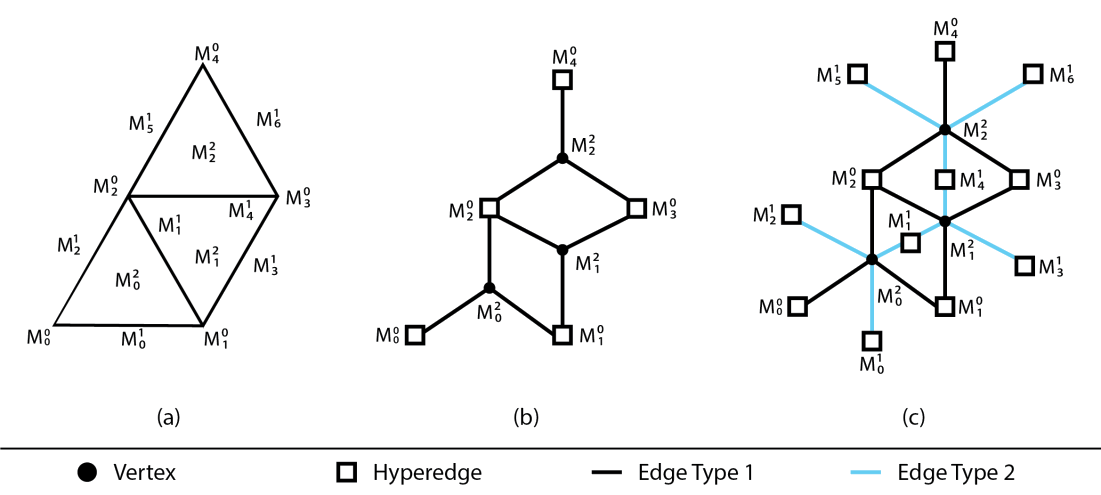
\includegraphics[width=.7\textwidth]{../figures/exampleMesh2Graph_backgroundless.png}
        \caption{Conversion from mesh (a) to N-graph (b),(c).}
      \end{figure}
     %Add higher order notes if there is room
    \end{block}
    \begin{block}{\centering Strong Scaling of Unstructured Mesh}
      %Discuss testing
      Tests were run on a one billion element mesh created and partitioned using:
      \begin{itemize}
      \item global ParMETIS part k-way to 8Ki($8*2^{10}$) parts and
      \item local ParMETIS part k-way from 8Ki to 128Ki, 256Ki, and 512Ki parts.
      \end{itemize}
      \begin{textblock}{2.3}(0,0.1)
        The initial partitions stats are: \\[1cm]

        Computing the 512Ki partition from 8Ki parts takes 16 seconds, followed by a migration that takes 131 seconds.
        
      \end{textblock}
      \begin{textblock}{2.5}(2.3,0)
      \begin{table}[!h]
        \centering
        \begin{tabular}{||c|c|c|c||}
          \hline
          Number of Parts &128Ki&256Ki&512Ki \\
          \hline
          Elements per part & 9,836 & 4,918&2,459  \\
          \hline
          Vertex imbalance & 1.13 & 1.18 & 1.53 \\
          \hline
          Element imbalance & 1.02& 1.02& 1.02\\
          \hline
        \end{tabular}
      \end{table}
      \end{textblock}
      \vspace{10cm}

      Running EnGPar on the three meshes results in:
      \begin{itemize}
      \item reducing element imbalance to 5\%
      \item reducing vertex imbalance to 5\% except for the 512Ki case which is reduced to 12\% imbalance.
      \item each run took less than 10 seconds to compute and migrate the data.
      \end{itemize}
      
      %Add results and images/graphs
      
    \end{block}
  \end{textblock}
  \begin{textblock}{5}(10.6,0)
    \begin{block}{\centering Overset Grids}
      Some unstructured mesh applications are accompanied with an overset grid.
      \begin{textblock}{2.7}(0,0.1)
        %More info about the overset grid applications
        These simulations add additional partitioning challenges such as:
        \begin{itemize}
        \item computational coupling between the meshes
        \item additional communication sources
        \item more...
        \end{itemize}

        %List assumptions?
        

      \end{textblock}
      \begin{textblock}{2.5}(2.5,0)
        %example image of the overset grid + mesh
        \begin{figure}
          \centering
          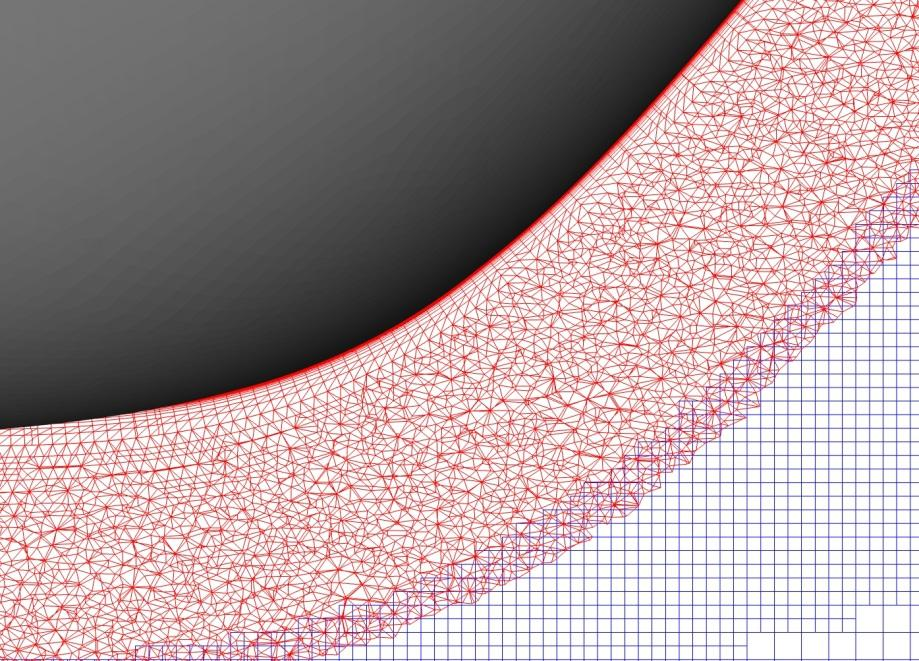
\includegraphics[height=.6\textwidth]{../figures/overset_grid.jpg}
          \caption{An unstructured mesh (in red) with \\an overset grid (in black).}
        \end{figure}
      \end{textblock}
      \vspace{14cm}

      
      %Describe the construction of the N-graph
      To construct the N-graph for these applications we:
      \begin{itemize}
      \item construct the vertices and hyperedges on the unstructured mesh any way for the application,
      \item add vertices for each element in the overset grid.
      \item add a second edge type that connects the graph vertices from the unstructured mesh to the graph vertices from the grid where the elements overlap.
      \end{itemize}

      %Add picture showing the conversion
      
    \end{block}
    
    \begin{block}{\centering FUN3D: Fluid dynamics simulations}
      FUN3D is a finite volume application that exhibits several partitioning problems beyond those found in standard finite element codes such as:
      \begin{itemize}
      \item the unstructured mesh is partitioned by mesh vertices.
      \item the simulation requires a ghost layer at part boundaries of neighboring elements.
      \item supports using an overset grid to interact with other simulations.
      \end{itemize}

      Traditional partitioning methods have trouble balancing these metrics. Also the vertex-based partition makes it difficult to use element-based mesh partitioning tools.

      %Discuss construction of N-graph
      For EnGPar, the construction of the graph on the mesh is as follows:
      \begin{itemize}
      \item create graph vertices from the mesh vertices
      \item create hyperedges for each mesh element
      \item create a pin for each mesh element surrounding the mesh vertex.
      \end{itemize}
      The ghost layer can be treated by accounting for the weight of the ghosted vertices in the diffusive iterations and the overset grid can be accounted for similar to the way as listed above.

      
    \end{block}
  \end{textblock}
\end{textblock}

\end{document}
